\documentclass[ALICE,manyauthors]{cernphprep}

\usepackage[comma,square,numbers,sort&compress]{natbib}
\usepackage{hyperref}
\usepackage{lineno}
\usepackage{multirow}
\usepackage{color}
\usepackage{rotating}
\usepackage{graphics}
\usepackage{soul}
\usepackage{bm}
\usepackage{hyperref}

\linenumbers

\newcommand{\dd}{\mathrm{d}}

\newcommand{\sigmastarpm}{\Sigma^{*\pm}}
\newcommand{\sigmastar}{\Sigma^*}
\newcommand{\antisigmastar}{\overline{\Sigma}^*}
\newcommand{\xistarzero}{\Xi^{*0}}
\newcommand{\xistar}{\Xi^*}
\newcommand{\antixistar}{\overline{\Xi}^*}
\newcommand{\snn}{\sqrt{s_{\mathrm{NN}}}}
\newcommand{\mpt}{\langle p_{\mathrm{T}}\rangle}
\newcommand{\dedx}{d$E$/d$x$}
\newcommand{\dndy}{d$N$/d$y$}
\newcommand{\mmass}{MeV/$\it{c}^2$}
\newcommand{\Tsallis} {L\'{e}vy-Tsallis} 
\newcommand {\reducedchisquare} {$\chi^{2}/\mathrm {ndf}$}
\newcommand {\gmom}   {\mbox{\rm GeV$\kern-0.15em /\kern-0.12em c$}}
\newcommand {\mmom}   {\mbox{\rm MeV$\kern-0.15em /\kern-0.12em c$}}
\newcommand {\Gmass} {\mbox{\rm GeV$\kern-0.15em /\kern-0.12em c^2$}}
\newcommand {\chisquare} {$\chi^{2}$}


\newcommand{\bmi}{\begin{minipage}}
\newcommand{\emi}{\end{minipage}} 

\newcommand{\sigst}{\ensuremath{\Sigma(1385)^{\pm}  \; }}
\newcommand{\xist}{\ensuremath{\Xi(1530)^0  \; }}

\newcommand{\meandNdeta}{\ensuremath{\langle$d$N_{\mathrm{ch}}$/d$\eta_{\mathrm{lab}}\rangle}}
\newcommand{\dndydpt}{${\rm d}^2N/({\rm d}p_{\rm T}{\rm d}y)$}

\newcommand{\sqrtS}{\ensuremath{\sqrt{s}}}
\newcommand{\PbPb}{\ensuremath{\mbox{Pb--Pb}}}
\newcommand{\pp}{\ensuremath{\mathrm {p\kern-0.05em p }}}
\newcommand{\pPb}{\ensuremath{\mbox{p--Pb}}}
\newcommand{\Pbp}{\ensuremath{\mbox{Pb--p}}}
\newcommand{\sqrtSnn}{\ensuremath{\sqrt{s_{\mathrm{NN}}}}}
\newcommand{\sqrtSE}[2][TeV]{$\sqrtS = #2\,\mathrm{#1}$}
\newcommand{\sqrtSnnE}[2][TeV]{$\sqrtSnn = #2\,\mathrm{#1}$}
\newcommand{\sqs}{\ensuremath{\sqrt{s} =  \;\; }}


\newcommand{\siglam}{\ensuremath{\frac{\Sigma^0}{\Lambda} \; }}
\newcommand{\sig}{\ensuremath{\Sigma^0  \; }}
\newcommand{\asig}{\ensuremath{\overline{\Sigma^0} \; }}
\newcommand{\gam}{\ensuremath{\gamma \; }}
\newcommand{\lam}{\ensuremath{\Lambda \; }}
\newcommand{\alam}{\ensuremath{\overline{\Lambda} \; }}
\newcommand{\meanpt}{ \ensuremath{\langle p_{\mathrm{T}} \rangle}} 


\newcommand{\pt}{\ensuremath{p_{\mathrm{T}\; }}}
\newcommand{\dEdx}{\ensuremath{\mathrm{d}E/\mathrm{d}x}}
\newcommand{\dndeta}{\ensuremath{\mathrm{d}N_{\rm ch}/\mathrm{d}\eta}}
\newcommand{\Raa}{\ensuremath{R_\mathrm{AA}}}
\newcommand{\Taa}{\ensuremath{T_\mathrm{AA}}}
\newcommand{\ncoll}{\ensuremath{N_{\mathrm{coll}}}}
\newcommand{\npart}{\ensuremath{N_{\mathrm{part}}}}

\newcommand{\MeVc}{\ensuremath{\mathrm{MeV}\kern-0.05em/\kern-0.02em c}}
\newcommand{\GeVc}{\ensuremath{\mathrm{GeV}\kern-0.05em/\kern-0.02em c}}
\newcommand{\GeVcSq}{\ensuremath{\mathrm{GeV}\kern-0.05em/\kern-0.02em c^2}}
\newcommand{\cLight}{\textit{c}}
\newcommand{\lumiUnit}{\ensuremath{{\rm cm}^{-2} {\rm s}^{-1}}}
\newcommand{\degree}{\ensuremath{^{\rm o}} }
\newcommand{\invmb}{\mathrm{mb}^{-1}}
\newcommand{\invmbps}{\invmb\mathrm{s}^{-1}}
\newcommand{\invub}{\mu\mathrm{b}^{-1}}
\newcommand{\invubps}{\invub\mathrm{s}^{-1}}
\newcommand{\invnb}{\mathrm{nb}^{-1}}
\newcommand{\invnbps}{\invnb\mathrm{s}^{-1}}
\newcommand{\invpb}{\mathrm{pb}^{-1}}
\newcommand{\invpbps}{\invpb\mathrm{s}^{-1}} % /pb/s    


\newcommand{\photon}{\ensuremath{\gamma}}
\newcommand{\wplus}{W$^{+}$}
\newcommand{\wminus}{W$^{-}$}
\newcommand{\zboson}{Z$^{0}$}
\newcommand{\eplus}{\ensuremath{{\rm e}^{+}}}
\newcommand{\eminus}{\ensuremath{{\rm e}^{-}}}
\newcommand{\epm}{\ensuremath{{\rm e}^{\pm}}}
\newcommand{\ee}{\ensuremath{{\rm e}^{+}{\rm e}^{-}}}
\newcommand{\mup}{\ensuremath{\mu^{+}}}
\newcommand{\mumi}{\ensuremath{\mu^{-}}}
\newcommand{\mupm}{\ensuremath{\mu^{\pm}}}
\newcommand{\mumu}{\ensuremath{\mu^{+}\mu^{-}}}
\newcommand{\rhop}{\ensuremath{\rho^{+}}}
\newcommand{\pip}{\ensuremath{\pi^{+}}}
\newcommand{\pim}{\ensuremath{\pi^{-}}}
\newcommand{\piz}{\ensuremath{\pi^{0}}}
\newcommand{\kap}{\ensuremath{{\rm K}^{+}}}
\newcommand{\kam}{\ensuremath{{\rm K}^{-}}}
\newcommand{\kashort}{\ensuremath{{\rm K}^{0}_{s}}}
\newcommand{\pbar}{\ensuremath{\rm\overline{p}}}
\newcommand{\ppbar}{\ensuremath{\rm p\overline{p}}}
\newcommand{\jpsi}{\ensuremath{{\rm J}\kern-0.02em/\kern-0.05em\psi}}
\newcommand{\psiP}{\ensuremath{\Psi^{\prime}}}
\newcommand{\upsi}{\ensuremath{\Upsilon}}
\newcommand{\upsiP}{\ensuremath{\Upsilon^{\prime}}}
\newcommand{\upsiPP}{\ensuremath{\Upsilon^{\prime\prime}}}
\newcommand{\qbar}{\ensuremath{\rm\overline{q}}}
\newcommand{\ubar}{\ensuremath{\rm\overline{u}}}
\newcommand{\dbar}{\ensuremath{\rm\overline{d}}}
\newcommand{\cc}{\ensuremath{{\rm c}\bar{{\rm c}}}}
\newcommand{\cL}{\textit{c}}

\newcommand{\red}{\textcolor{red}}
\newcommand{\blue}{\textcolor{blue}}
\newcommand{\magenta}[1]{\color{magenta}{#1}\color{black}}
\newcommand{\rmSigma}          {\mbox{$\mathrm {\Sigma}$}}

%
\begin{document}%

%%%%%%%%%%%%%%%  Title page %%%%%%%%%%%%%%%%%%%%%%%%
%
\begin{titlepage}
%

\PHyear{2018}
\PHnumber{D1.0}   % required, will be obtained from PH
\PHdate{\today}  % required, will be obtained from PH


\title{$\Sigma^{0}$ and $\overline{\Sigma}^{0}$ Production in pp Collisions at $\sqrt{s} = 7$ TeV }

\ShortTitle{$\Sigma^{0}$ in pp at $\sqrt{s} = 7 $ TeV}   % appears on right page headers

\author{PC: A.~Borissov,  A.~Badala, I.-K.Yoo \\
IRC:} 

\Collaboration{ALICE Collaboration\thanks{See Appendix~\ref{app:collab} 
for the list of collaboration members}}
\ShortAuthor{ALICE Collaboration} % appears on left page headers, do not change


\begin{abstract}
%%%%%%%%%%%%%%%%%%%%%%%%%%%% Abstract %%%%%%%%%%%%%%
The first measurements of $\Sigma^{0}$ and $\overline{\Sigma}^{0}$ baryons'
transverse momentum ($p_{\rm{T}}$) spectra, integrated yields and mean $p_{\rm T}$ 
in pp collisions at the LHC are reported. The $\Sigma^{0}$ 
($\overline{\Sigma}^{0}$) signal is reconstructed via the $\Lambda$
($\overline{\Lambda}$) + $\gamma$ decay channel by invariant mass analysis.
The $\Lambda$ ($\overline{\Lambda}$) baryon is reconstructed by its decay
into p + $\pi^{-}$ ($\overline{ \rm{p}} + \pi^{+}$), while the photon is detected
exploiting the unique capability of the ALICE detector to measure low energy
photons via conversion into e$^{+}$e$^{-}$ pairs.
The yield of $\Sigma^{0}$ is compared to that of the
$\Lambda$ baryon, which has the same quark content but different
isospin. These data contribute to the understanding of hadron production
mechanisms and provide a reference for constraining QCD-inspired models and
tuning Monte Carlo event generators such as PYTHIA. \\

%%%%%%%%%%%%%%%%%%%%%%%%%%%%%%%%%%%%%%%%%%%%%%%%%%%%
\end{abstract}

\end{titlepage}
\setcounter{page}{2}

 \tableofcontents  

\newpage

%%%%%%%%%%%%%% Chapter 1 : Introduction %%%%%%%%%%%%
 \section{Introduction}
 \label{sec:intro}

The study of strange baryons and their resonances in proton-proton collisions provides a reference for tuning QCD 
inspired event generators and contributes to the understanding of strangeness production mechanisms. Colliding projectiles initially 
contain no strange valence quarks indeed and therefore all strange particles are created in the 
collisions. In particular, $\Sigma$~measurements can help to understand production mechanisms of baryons with non-zero 
isospin. These are an important complement of the Lambda data as these particles have similar mass 
($m_{\Sigma} - m_{\Lambda} \sim$~77~MeV) and equal quark content (uds), but different isospin value 
($I_{\Lambda}$ =0, $I_{\Sigma}$ =1)~\cite{cite:PDG}. Furthermore a yield ratio of \sig to \lam can provide 
a hint to understand a charge and/or isospin independency of the $\Sigma^\pm$ and $\Sigma^0$ due to the same $I(J^p)$, 
analogy to the yield ratio of $\pi^0$/$\eta$\red{~\cite{cite:pi_eta}}.

All \lam (\alam) measurements include a feed-down from \sig (\asig). In fact, the main decay of the \sig (\asig) is the 
electromagnetic one (\sig (\asig)$\to $ \lam (\alam) + \gam) with a 100~\%~branching ratio. Usually this feed-down contribution 
is not considered for the \lam (\alam) spectrum and as a consequence, model predictions for \lam (\alam) baryons are 
compared with data including secondary \lam (\alam) originated from \sig (\asig)\red{~\cite{cite:lamda_model}}. 
Thus the measurement of the \sig (\asig) spectrum enables us to estimate the contribution of the secondary \lam (\alam) 
in the hyperon spectrum. Furthermore, the \sig production rates can be also an important measure to correct the \pt spectra of
proton, pion and photon with taking into account the feed-down contributions from \sig.

Comparison of hyperon data with models as  PYTHIA~\cite{cite:pythia6} and EPOS~\cite{cite:EPOS3} permits 
to investigate their production mechanism. In particular, at LHC energies a significant disagreement was observed in 
\pt~spectrum of \lam between PYTHIA6 Perugia 2011~\cite{cite:pythia6} predictions and measurements of 
ALICE~\cite{cite:DDChin-Lam} and ATLAS~\cite{cite:ATLAS-Lam-pp-2011} experiments. 
In this respect, the measurement of the \pt spectrum of  \sig and the ratio of \sig to \lam at the LHC energy
are fundamental for the tuning of the models and to understand the hadronic mechanism 
processes.

In this paper the first measurement of the \sig (\asig) transverse momentum spectrum and its integrated yield measured 
at mid-rapidity with ALICE detector in inelastic pp collisions at $\sqrt{s} =$7 TeV are presented and compared
with the \lam results in the same collisions. This enriches the existing data set limited until now to low energy collisions results. 

%%%%%%%%%%%%%% Chapter 2 : Experimental setup %%%%%%%%%%%%
 \section{ Experimental setup and event selection}
 \label{sec:exp}
 
Since a complete and detailed description of the ALICE detector and of its performance 
 during the LHC Run 1 (2010-2013) can be found in refs \cite{cite:ALICE,cite:ALICEPerformance}, 
 we briefly outline only two sub-detectors utilized for \sig analysis:
Inner Tracking System (ITS) and the Time Projection Chamber (TPC) below. 

Vertex reconstruction and tracking in the central-barrel  and charged-hadron identification are performed with the
Inner Tracking System (ITS)~\cite{cite:ALICE} and the Time-Projection Chamber (TPC)~\cite{cite:TPC}, 
which are located inside a solenoidal magnet providing a magnetic field of 0.5 T parallel to the LHC beam axis. 
The ITS is composed of six cylindrical layers of silicon detectors, located at radii between 4 and 43 cm from
the nominal beam axis with covering a pseudo-rapidity range of $|\eta|<0.9$ and the full azimuth. The two innermost layers
consist of Silicon Pixel Detectors (SPD), the two intermediate layers of Silicon Drift Detectors (SDD) and the two outermost
layers of Silicon Strip Detector (SSD). The spatial resolution of the ITS enables measuring the distance of closest approach 
(DCA) of tracks to the primary vertex with a resolution better than 75~$\mathrm{\mu}$m in the transverse plane for \pt $>$ 
1 GeV/$c$ in pp collisions~\cite{cite:Xi_c}. 
The Time Projection Chamber (TPC) is a large (90 m$^3$)
cylindrical gaseous detector filled with a mixture of Ne/CO$_2$ /N$_2$ (85.7/9.5/4.8\%). It covers radially between 85 and 250 cm from the 
beam axis and a pseudo-rapidity range of $|\eta| < 0.9$ over the full azimuth, and provides track reconstruction with up to 
159 space points, with a spatial resolution of 500~$\mu$m along the beam direction and in the transverse direction for tracks 
with $\eta$=0~\cite{cite:TPC}. In addition, it enables particle identifications via the measurement of the specific 
ionization energy loss (d$E$/dx) with a resolution of approximately 5.2\% in pp collisions~\cite{cite:ALICEPerformance}.
%The combined acceptance of the ITS and TPC in rapidity ($y$) is $|y|<0.9$.

The data sample analyzed in this paper was recorded during the LHC pp run
at \sqs 7 TeV in 2010 (\red{only ? or - 2013?}) using a magnetic field of 0.5 T, with both field polarities 
and a minimum-bias (MB) trigger which requires at least one hit in either SPD or the one of the V0 detectors. While 
SPD covers $|\eta|<2.0$, the two V0 detectors, each consisting of scintillator tiles, are installed on both sides of the interaction 
point and cover -3.7 $< \eta <$ -1.7 and 2.8 $< \eta <$ 5.1~\cite{cite:ALICE2010-ChargeMult,cite:pi0-2012,
cite:ALICE2015-InclPhot-pp}.

These \red{(What is 'these'?)} are used for triggering \red{(Is it the same to $f_{inel}$, which must be same to the $MB_{OR}$ = INEL?}) 
and for rejecting beam-gas interactions \red{(What is it?)}. 
Due to the low luminosity of this \red{(Where can I find it?)} data taking a high-efficiency ( 85.2 \%~\cite{cite:ALICE2015-InclPhot-pp})  
MB trigger (\red{It is NOT the MB, but $MB_{OR}$!}) was used. 
The contamination from beam-induced
background is removed offline by using the timing information and correlations \red{(Which correlation?)} in
the V0-A,V0-C and SPD detectors, as discussed in detail in ref.\cite{cite:ALICEPerformance} \red{(Is this related to N$_{offlinetrigger}$? But how?)}.  
The probability of collision pileup per triggered event was below 3 \%~\cite{cite:ALICE2015-InclPhot-pp}\red{(How is it treated? Is it also taken into 
account for the final N$_{norm}$), but how?}. A total amount of about 500 million MB events has been utilized for the analysis. 

\red{Events used for the data
analysis are further required to have just one reconstructed primary vertex (PV),
events containing more than one distinct  vertex are tagged as pileup and are discarded. 
The PV is determined by tracks reconstructed in the ITS and Time Projection Chamber (TPC), 
and track segments in the SPD~\cite{cite:ALICEPerformance}. 
MB events are selected when 
the  PV is positioned along the beam axis within $\pm$10 cm from the center of the ALICE detector
The vertex reconstruction efficiency is 92.8 \%~\cite{cite:ALICE2015-InclPhot-pp}.}
These are all unnecessarily reapeated even with confusion!

\blue{Question: 
in~\cite{cite:ALICE2015-InclPhot-pp}, MB$_{OR}$ = INEL = at least one hit at SPD OR one of V0s\\
NSD = an additional condition of coincidence of two V0s = MB$_{AND}$\\
What was used? MB$_{OR}$ or MB$_{AND}$? \\
MB$_{AND}$/MB$_{OR}$ = 0.873
in~\cite{cite:NSD, cite:Xi_c} $f_{inel}$ = trigger efficiency for INEL = 87\%, $f_{vtx}$ = vertex reconstruction within $\pm$10cm = 88\%\\
What is then $N_{in}$ and $N_{offilinetrigger}$? Nowhere I can find it.\\
what is the relation between $N_{norm}$ and $N_{MB}$?}

%%%%%%%%%%%%%%%%%%%%%%%%%%%%%%
 \section{Data analysis}
 \label{sec:analysis}

\sig  were reconstructed by its electromagnetic decay 
( \sig (\asig) $\to $ \lam (\alam) + \gam \;) which has a 100 \% branching ratio.  
\red{The main feature of this decay is the low energy of the energy of the emitted photon
$\approx 100$ MeV \blue{(any reference? Why is it relevant?)}.}
The Photon Conversion Method (PCM) in the central tracking system was used for photon identification 
employing the ITS and the TPC~\cite{cite:ALICEPerformance,cite:ALICE-DirPhot2016,cite:pi0-2012}.
It  reconstructs and identifies  the vertices (V0$_{\gamma}$) of photon conversions to $e^+ e^-$ pair generatedi in the
material of the inner detectors. For ALICE detector the  probability of photon conversion in the central tracking system is about 0.08 and the 
reconstruction efficiency  is about $0.67$ \cite{cite:pi0-2012}. Reliability of the method is based on the 
good agreement of the actual material budget and the simulated one~\cite{cite:ALICEPerformance}. 
Then both the decay products of the \sig were identified as secondary vertices (V0): $V0_{\Lambda}$ of 
the weak decay   $ \lam (\alam) \to p (\bar p) + \pi^+ (\pi^-)$ and $V0_{\gamma}$ of the photon conversion
during tracking procedure.

In the PCM analysis,  photons are reconstructed as vertices (V0$_{\gamma}$) of  electron and positron 
pair~\cite{cite:pi0-2012,cite:ALICE2014-pi0-pp-pPb-2.76TeV,cite:ALICE-DirPhot2016,cite:ALICE-pi0eta-2018}.
The tracks for $e^-$ ($e^+$) candidates are basically selected if: (1) $|\eta| <0.9$, (2) \pt $>$ 0.05 GeV/c, 
(3) the ratio of the number of reconstructed to findable TPC  clusters is larger than 0.35.
For the particle identification of $e^-$($e^+$) tracks, the specific energy loss of electrons (positrons) in the TPC
was required to be within a band between $-6\sigma_{e}$ and $7\sigma_{e}$ around the
average d$E$/dx-value depending on \pt, where $\sigma_{e}$ is a standard deviation
of the measured d$E$/dx distribution for $e^-$($e^+$).
In addition,  in order to reduce pion and kaon contaminations by rejecting the tracks with $|$d$E$/dx$|<1\sigma_{\pi, K}$ 
for \pt $<$ 0.5 GeV/c, where $\sigma_{\pi, K}$ are the standard deviations of measured d$E$/dx 
distribution for pions ($\sigma_{\pi}$) and kaons ($\sigma_{K}$), respectively. 

To select photons among all secondary vertices, further selection was performed on the level of the 
reconstructed  V0$_{\gamma}$~\cite{cite:ALICE-DirPhot2016,cite:pi0-2012}. 
To remove $\pi^0$ and $\eta$ meson Dalitz decays, the transverse distance \red{(why only R$_T$?)} 
of V0$_{\gamma}$ from PV have to be larger than 5 cm and smaller than 180 cm due to the V0 reconstruction 
procedure. Finally, the photons only with \pt $> 0.020$ GeV/c and $|\eta| <0.9$ are accepted.
Additional cuts of $q_{\rm{T}} = p_e \sin{\Theta_{\gamma,e}}<0.06$ GeV/$c$, where $p_e$ is electron momentum and
$\Theta_{\gamma,e}$ is the angle between  $\gamma$ momentum ($p_\gamma$) and electron momentum
~\cite{cite:ArPod}, and $\Psi_{pair} < 0.20$, where $\Psi_{pair}$ is the angle between the plane perpendicular to 
the magnetic field ($x-y$) plane and the plane of the $e^-(e^+)$ pair~\cite{cite:ALICE-pi0eta-2018}
are applied for increasing the purity of $e^-(e^+)$ from $\gamma$.

To select \lam from $\Sigma^0$, the similar selection-criteria of the secondary vertex ($V0_{\Lambda}$) used 
in~\cite{cite:DDChin-Lam,cite:lambda_pp,cite:Lam-PLB14} with exploiting the weak decay topology
of \lam(\alam)$ \to p \pi^{-} (\bar{p} \pi^{+})$ (branching ratio of 63.9\% and decay length of
$c\tau = 7.89$ cm~\cite{cite:PDG}), is applied. The distance of closest approach (DCA) between 
positive and negative tracks from V0$_\Lambda$ and PV \red{(Why PV?)} was selected to be larger 
than 0.06 cm, and the cosine of the pointing angle $\Theta$ between the sum of daughter momenta and 
the line that connects the PV and V0$_\Lambda$, was requested to be greater than 0.993. The transverse 
distance between V0$^\Lambda$ and PV is requested to be between 0.5 and 180 cm. An 
Armenteros-Podolanski cut on \lam: $0.01 < \alpha < 0.17$ and $0.2 < |q_{\rm{T}}| < 0.9 $ 
was applied, where $\alpha_{\Lambda}  = |\frac{ p_l^{p} - p_l^{\pi}}{ p_l^{p} + p_l^{\pi} }  |$, where $p_l^i$ 
is the longitudinal momentum of a particle $i$ (p or $\pi$) 
with respect to the $\Lambda$ momentum direction, $q_{\rm{T}}$ corresponds to transverse momentum 
of proton with respect to the $\Lambda$ momentum. The $\Lambda$ invariant mass ($M_{\rm{p}\pi}$) was selected 
within the interval of 1.110 $< M_{\rm{p}\pi}  < 1.120$ GeV/$c^2$ to reduce the amount of combinatorial 
background of \sig invariant mass peak. Note, the nominal \lam mass ($m_\Lambda$) with its uncertainty is m$_\Lambda=1115.683 \pm 0.006$~\cite{cite:PDG}.

\begin{table}[h!]
\centering
\begin{tabular}{c| cc| c}
 & $\gamma$ & $\Lambda$ & $\Sigma^0$ \\
\hline\noalign{\smallskip}
$p_{\rm{T}}$ & $> 0.020$ & $>0.4$ & $> 1.1$ \\
$|\eta|$ & $< 0.9$ & $< 0.5$ & $< 0.5$ \\
% cos$\Theta$ &  & $< 0.993$ &  \\
$\alpha$ & - & (0.01, 0.17) & $>0.6$ \\
$q_{\rm{T}}$ & $< 0.06$ & (0.2, 0.9) & $< 0.12$ \\
\hline\noalign{\smallskip}
\end{tabular}
\caption{The final selection criteria of \sig and its daughter particles.}
\label{tab:selection}    
\end{table} 

In order to enhance the significance of the \sig signal, softer cuts on \lam selection than those used in 
\lam~\cite{cite:lambda_pp,cite:Lam-PLB14} and the additional phase-space cuts on \sig as
$\alpha  = |\frac{ p_l^{\gamma} - p_l^{\Lambda} }{ p_l^{\gamma} + p_l^{\Lambda} } |>0.6$ and $p_{\rm{T}} < 0.12$,
\red{($p_T$ ? or $q_T$?)} are applied. Furthermore the rapidity range ($|y|$ \red{(not $|\eta|$?)}) less 
than 0.5 is selected for comparing directly with $\Lambda$ results. The final ranges of the criteria are summarized 
in Table~\ref{tab:selection}.

%%%%%%%%%%%%%%%%%%%%%%%%%%
 \subsection{Signal extraction} 
 \label{subsec:signal}

The $\Sigma^{0} + \overline{\Sigma}^{0}$ signals were extracted from invariant-mass 
distributions in each \pt-bin of \sig for the range of 1.1 up to 8 GeV/$c$. For the estimates of raw yield of
the signal, a Gaussian function added to a third-order polynomial is applied to describe the signal and 
background for the range of 1.160 $< M_{\Lambda\gamma}<$ 1.230 GeV/c$^2$ in each \pt-bin. Examples of 
invariant mass distribution are presented in Fig.~\ref{fig:InvMassSigma0} for two different \pt-bins.

\begin{figure}[h!]
\hspace*{-1.0cm}  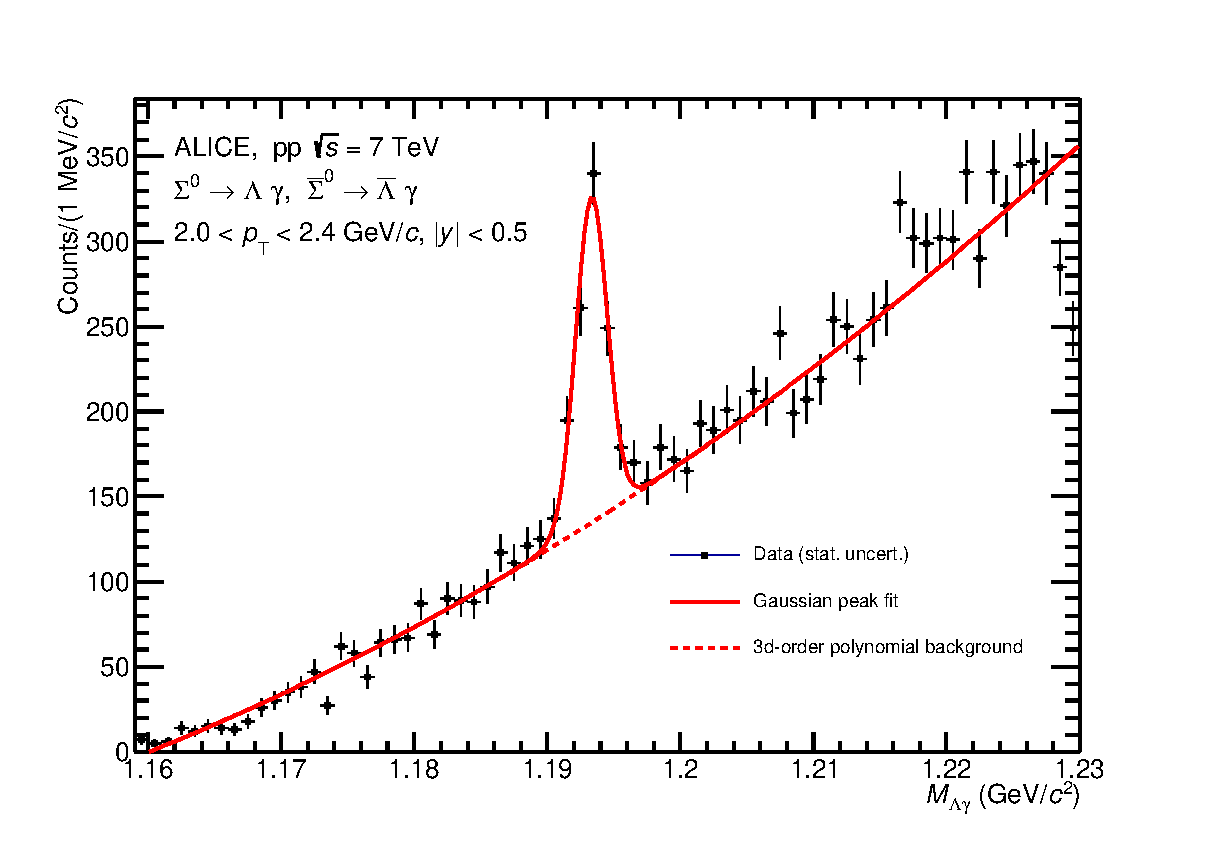
\includegraphics[width=9.cm]{Figure/10jan18Minvbin3.eps}
\hspace*{-1.0cm}  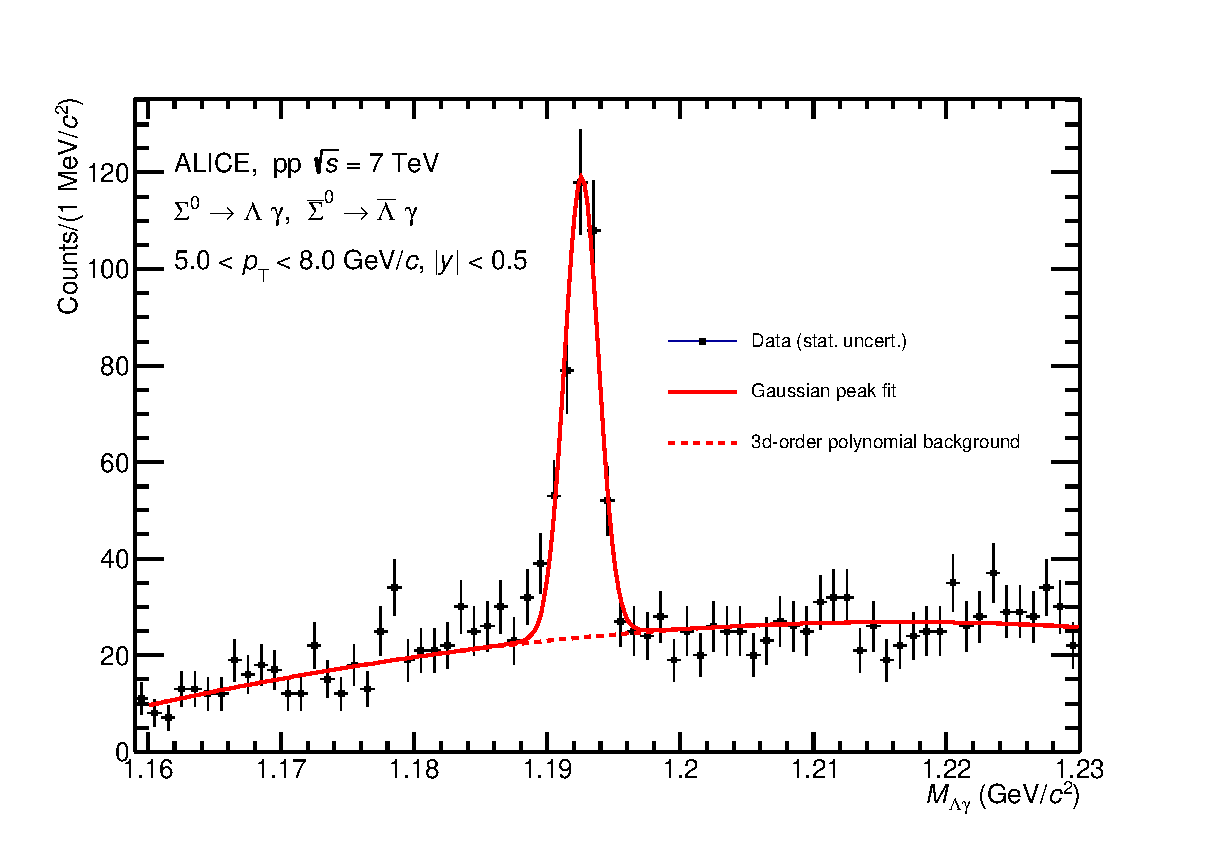
\includegraphics[width=9.cm]{Figure/10jan18Minvbin8.eps}
\caption{
Invariant mass distributions of $\Lambda\gamma$ and $\bar \Lambda \gamma$ pairs in \pt bins 1.6 -- 2.0 
and 4.0 -- 5.0 GeV/c. The solid and dashed curves indicate a fit to the data using a third-order polynomial 
function with and without a Gaussian peak for the signal and background description, respectively.
}
  \label{fig:InvMassSigma0}
\end{figure}

The mean value ($M_{\Lambda \gamma} = 1192.94 \pm 0.035 MeV/\rm{c}^2$) of the 
$\Sigma^0+ \overline{\Sigma}^{0}$ invariant masses from the fit results in all \pt-bins agrees
well to the PDG value~\cite{cite:PDG}: 1192.642 $\pm$ 0.024 MeV/c$^2$.
The standard deviations of the \sig signals extracted from the fits to data are about 2.2 MeV for 
$1.1 <$ \pt $< 1.6$ GeV/$c$ and about 1.2 MeV for \pt$>$ 2 GeV/$c$, which are in a good agreement 
with the ones estimated by the fits to the simulated distributions. \red{(How about then between 1.6 -- 2 GeV/c?)}
The increase of the width at low \pt is mainly due to the low-energy photons.

The raw yield is obtained by integrating the Gaussian signal function in the region $\pm 3$ standard deviation 
in each  \pt  bin. The statistical uncertainties on the raw yields range between 3-6\%.
The different approaches with various signal and background estimations and 
the calculations of \sig yields are discussed for the systematic uncertainties in section~\ref{subsec:systematics}.

%%%%%%%%%%%%%%%%%%%%%%%%%%
 \subsection{Corrections and normalization}

By using the PYTHIA6 Perugia-2011 event generator~\cite{cite:pythia6}
and the GEANT~3.21 package~\cite{cite:GEANT}, the \sig signals are reconstructed in each \pt
from a generated sample of about 542 million MB pp events, and the correction factors ($A\times\epsilon$) are 
estimated from the ratio between the number of reconstructed and generated \sig hyperons 
in the same \pt and rapidity interval. The \pt distribution of correction factors multiplied by branching 
ratios (B.R.) for \sig is shown in Fig.~\ref{fig:efficiency}. The correction factors for \sig and \asig 
are checked, respectively, and are consistent between each other in the measured \pt-interval between 
1.1 and 8 GeV/$c$. Raw yields are thus corrected for the geometrical acceptance and the reconstruction efficiency
(A $\times$ $\epsilon$) of the detector with taking into account the branching ratio of \lam decay.

\begin{figure}[bt]
\centering  
      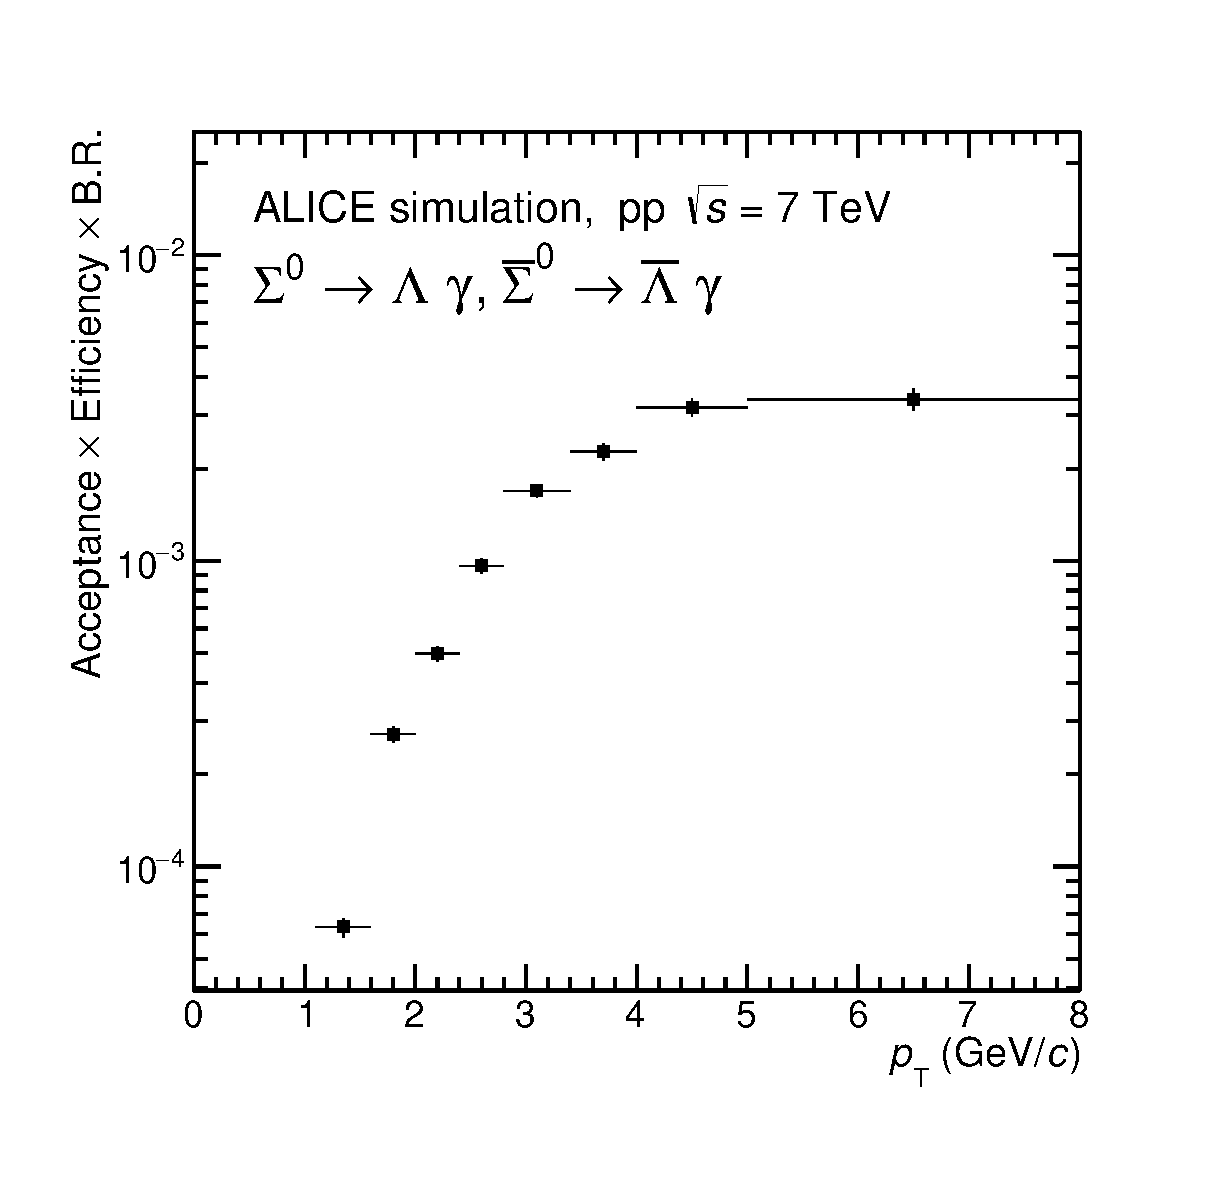
\includegraphics[width=10.cm]{Figure/2017oct31-Sigma0-AccEffi.eps}

  \caption{The geometrical acceptance and the reconstruction efficiency
  (A $\times$ $\epsilon$) multiplied by B.R. for $\Sigma^{0}$ in $ |y| <$ 0.5 for 
  MB events, obtained with PYTHIA6 Perugia-2011 event generator~\cite{cite:pythia6}
  \red{(\asig must be removed in the plot!)}.
  Only statistical uncertainties are shown.\red{(why? How much is the systematic uncertainties for each \pt?
  - nowhere explained even also not in \ref{subsec:systematics}.)}}
  \label{fig:efficiency}
\end{figure}

\red{The MB spectrum was normalized to the number of 
$N_{norm}$ events after applying the correction factors for trigger efficiency and event 
selection including primary vertex reconstruction and rejection of pileup events
It was done analogous to the approach implemented in PCM package which 
was already  used in several publications of ALICE~\cite{cite:ALICE2015-InclPhot-pp,cite:ALICE-DirPhot2016} .
All those corrections result in a total scaling factor of 0.922 for the calculation of the total  
number of events used in Eq.~\ref{eqn:funclevy}.}
%\blue{ (See Appendix~\ref{app:MBnorm})}.}

\red{The MB spectrum was normalized to the number of
$N_{norm}$ events after applying the correction factors for trigger efficiency and event selection including primary vertex reconstruction and rejection of pileup events.
The yield of \sig as a function of \pt is after background subtraction $N^{\Sigma^0}$:
\begin{equation}
\frac{d^2N}{\rm{d}p_{\rm{T}}\rm{d}y } =   \frac{1}{N_{MB}} \frac{N^{\Sigma^0}}{\Delta y \Delta \pt}
\frac{ f_{vtx} \times f_{inel}}{A \epsilon} ,
\label{eq:normMB}
\end{equation}
where
$N_{MB} = N_{in} - N_{OfflineTrigger}$  - trigger hits in either of two VZERO detectors,
the factor $f_{vtx}$ is the fraction of triggered events for which a good primary vertex is found,
$ f_{inel}$ is the fraction of inelastic collisions that fulfill the trigger conditions.
It was done analogous to the approach implemented in PCM package which
was already  used in several publications of ALICE~\cite{cite:ALICE2015-InclPhot-pp,cite:ALICE-DirPhot2016} .
All those corrections result in a total scaling factor of 0.922 for the calculation of the total number of events used in Eq.~\ref{eqn:funclevy}.}

\blue{Question: 
in~\cite{cite:ALICE2015-InclPhot-pp}, MB$_{OR}$ = INEL = at least one hit at SPD OR one of V0s\\
NSD = an additional condition of coincidence of two V0s = MB$_{AND}$\\
What was used? MB$_{OR}$ or MB$_{AND}$? \\
MB$_{AND}$/MB$_{OR}$ = 0.873
in~\cite{cite:NSD, cite:Xi_c} $f_{inel}$ = trigger efficiency for INEL = 87\%, $f_{vtx}$ = vertex reconstruction within $\pm$10cm = 88\%\\
What is then $N_{in}$ and $N_{offilinetrigger}$? Nowhere I can find it.\\
what is the relation between $N_{norm}$ and $N_{MB}$?}

%%%%%%%%%%%%%%%%%%%%%%%%%%
 \subsection{Systematic uncertainties} 

\label{subsec:systematics}

The total \sig systematic uncertainty is determined by four general sources: 
\begin{equation}
 \sigma_{syst} = \sqrt{ \sigma_{\gamma}^2 + \sigma_{\Lambda}^2 + \sigma_{\Sigma^0}^2  + \sigma_{mat}^2 },
 \label{eq:systematic}
\end{equation}
where $\sigma_{\gamma}$ and $\sigma_{\Lambda}$ are the relative systematic uncertainties for the photon ($\gamma$) 
and $\Lambda$ ($\bar{\Lambda}$) selections for the \sig (\asig) resonance, respectively, while $\sigma_{\Sigma^0}$ 
and  $\sigma_{mat}$ are the systematic uncertainty due to the extraction of \sig + \asig signals and the limited 
knowledge of the material budget for the conversion photon, relatively. As two V0s for reconstruction of 
\sig + \asig resonances are independently analyzed with the photon conversion ($\gamma \to e^+ e^-$) and 
the weak decay ($\lam \to  \rm{p} + \pi^-$ and $\alam \to \rm{\bar{p}} + \pi^+$), the corresponding systematic 
uncertainties are fully independent. \red{Note, that quite low yield of the detected \sig + \asig limits the possibility 
of the extraction of several components of the systematic uncertainties which were investigated in
stand-alone analysis of \lam and isolated photon production with much larger statistics.(Do we need this argument? For what?)}

The main sources of systematic uncertainties for \lam selection are following:
the pointing angle $\Theta$, V0$_{\Lambda}$ position, DCA between the \lam decay products, the ratio of 
 the number of the reconstructed to the findable TPC clusters and, \red{the difference between 
 the proper lifetimes estimated from the difference $L \frac{m^{\Lambda} - m^{K^0_s}}{p}$,
where $L$ is defined as the distance between primary and  V0$^{\lam}$ vertex and
$p$ is its momentum.(What is it? It was not mentioned before at all! The uncertainties of 
PID of daughter particles MUST be included, instead.)}
The relative systematic uncertainties estimated in this analysis for the \lam identification 
vary between 3 to 11 \% depending \pt, see Table~\ref{tab:sys}, and are consistent
with the ones estimated for \lam results in~\cite{cite:DDChin-Lam,cite:lambda_pp}.

The main source of the photon reconstruction uncertainty for PCM is determined by the identification
of $V0^{\gamma}$. The uncertainty of identification of $e^+$ and $e^-$ tracks is estimated with varying 
the restrictions of $\sigma_e$ in the TPC relative to the nominal d$E$/dx, and the contamination criteria
($\sigma_{\pi,\rm{K}}$) of pions and kaons~\cite{cite:pi0-2012}. The limits of the accepted
$V0^{\gamma}$ were also varied to evaluate its stability. The contribution of photon selection 
systematic uncertainty varies 4 to 12 \% also depending \pt. 

The systematic uncertainty of \sig+\asig yield extraction is estimated by 
 varying the conditions of the background subtraction and raw-yield calculation of the invariant mass peaks
shown in Fig.~\ref{fig:InvMassSigma0}. The various combinations of the signal and the background 
distributions estimated by a mixed-event ($e^+e^-$ pairs from different events) and a second-order polynomial, 
and the bin-counting method are applied for the for raw-yield extraction. The systematic uncertainties of 
raw-yield extraction range 2 to 10.5 \%. 

All systematic uncertainties are summarized in Table~\ref{tab:sys} for all \pt, and the mean value of the total systematic 
uncertainty averaged over all $\pt$-bins is 11.84 \%. 

\begin{table}[h!]
\centering
\begin{tabular}{lccccccccc}
\hline\noalign{\smallskip}
$\sigma_{\Lambda}$                &  3 - 11 \% \\
$\sigma_{\gamma}$                &  4 - 12  \% \\
$\sigma_{\Sigma^0}$                 & 2 - 10.5  \% \\ 
Material budget       & 4.5 \% \\
\hline\noalign{\smallskip}

Total \%                 & 8 - 17 \\

\hline\noalign{\smallskip}

\end{tabular}
\caption{Systematic uncertainties in \sig yield. The single valued uncertainties are \pt independent. 
Values given in ranges correspond to the minimum and maximum uncertainties.
}
\label{tab:sys}    
\end{table} 

%%%%%%%%%%%%%% Chapter 3 : Results and discussion %%%%%%%%%%%%
 \section{Results and discussion}
 \label{sec:results}

 \subsection{Transverse momentum spectrum} 
 \label{subsec:pT}

The corrected yield at mid-rapidity (d$N$/d$y$) of (\sig+\asig)/2 per event in \pt produced from inelastic pp collisions 
at 7 TeV is shown in Fig.~\ref{fig:spectra}. The measurements span the \pt range is from to 1.1 to 8 GeV/$c$. 
It was checked that the spectra obtained separately for \sig and \asig are equal inside the uncertainties.

\begin{figure}[h!]
\centering
 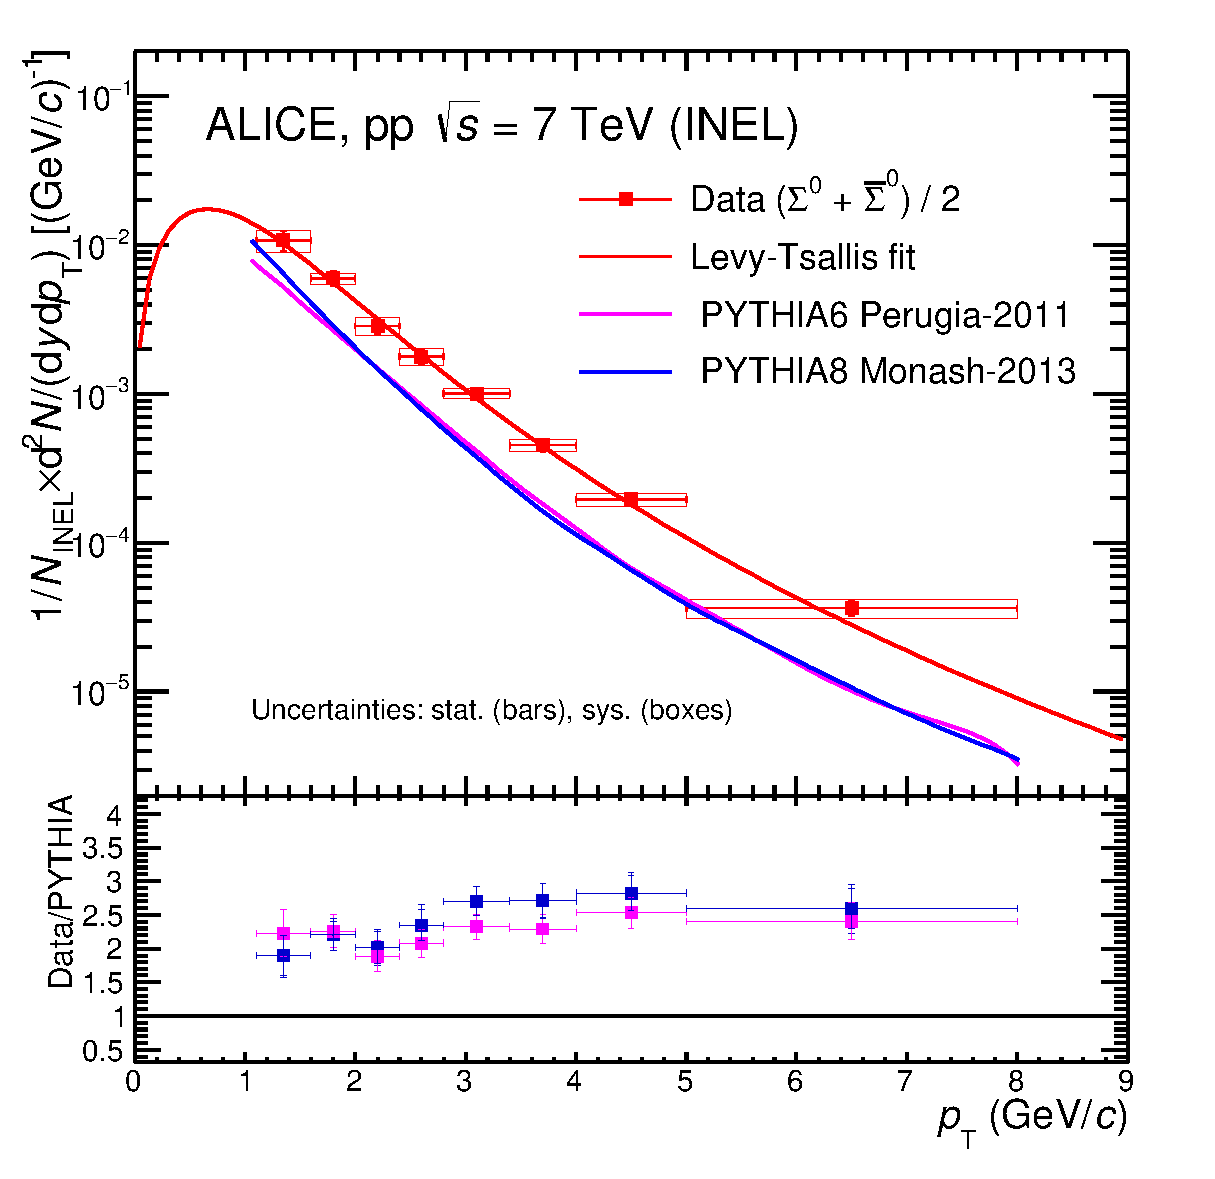
\includegraphics[width=8.0cm]{Figure/CM-6feb18-Data-LTfit-Pyt6-Pyt8.eps}

  \caption{(Top panel) Transverse momentum spectrum of both (\sig+\asig)/2 in  the rapidity range $|y|<0.5$. 
  Statistical (bars) and systematic (boxes) uncertainties are included. The solid line
  represents L\'{e}vy-Tsallis fit, the dashed and dot-dashed lines \red{(The figure must be updated for w/b (no color))} 
  represents the spectrum from PYTHIA6 Perugia-2011~\cite{cite:pythia6} and PYTHIA-8 Monash-2013
  ~\cite{cite:PYTHIA-8-Monash-gener} generators.
  (Bottom panel) Ratio of (\sig+\asig)/2 yield to the simulated ones for each generator in \pt.
  }
 \label{fig:spectra}
\end{figure}

The spectra are fitted with a L\'{e}vy-Tsallis function~\cite{cite:Tsallis}, 
\begin{equation}
\frac{1}{N_{norm}}\frac{\mathrm{d}^2N}{\mathrm{d}p_{\mathrm{T}}\mathrm{d}y} = p_{\mathrm{T}} 
\frac{\mathrm{d}N}{\mathrm{d}y} \frac{(n-1)(n-2)}{nC[nC+m_{0}(n-2)]}\left[1+
\frac{\sqrt{p_{\mathrm{T}}^2+m_{0}^{2}}-m_{0}}{nC}\right]^{-n},
\label{eqn:funclevy}
\end{equation}
where $N_{norm}$ is the number of MB events after the application of the correction factors, 
\red{(How and where is the N$_{norm}$ defined? Isn't it the N$_{INEL}$, as labeled in Fig.~\ref{fig:spectra}??)}
$m_0$ is the PDG value of $m_{\Sigma^0}$~\cite{cite:PDG}. Free parameter of the fit are the $n, C$ and \dndy, which represents 
the particle yield per unit of rapidity. This fit function is widely used to describe all identified particle spectra in pp 
collisions\cite{cite:Xi_pp,cite:KphipPb, cite:lambda_pp}, and to extract the integrated total yield for all \pt.

Finally, the integrated yield at mid-rapidity for \sig of d$N$/d$y = 0.0256  \pm 0.0083_{(total)} = 0.0256   \pm 0.0038_{(stat)} 
\pm 0.0047_{(syst)} \pm 0.0057_{(extrap)}$ is obtained from L\'{e}vy-Tsallis fit of Fig.~\ref{fig:spectra}.
The uncertainty (not shown \red{(why?)}) related  to the overall normalization to inelastic events (or cross section) 
is fully correlated \red{(with what?)} and it amounts to +7.3\% and -3.5 \%~\cite{cite:ALICE-inelasticXsection,cite:Xi_pp}.
The value of the mean $\mpt$ of  \sig was taken from the result of the fit without the uncertainty on material 
budget \red{(why? What is then with $\sigma_{mat}$ as shown in Table~\ref{tab:systematic}?
Isn't it included to the $\sigma_{syst}$?)}: \meanpt = 1.161 $\pm$ 0.085 ($\pm 0.076_{stat} \pm 0.038_{syst}$). 

The values of \dndy~and $\mpt$ were calculated by using the experimental 
spectrum in the measured \pt-range and the L\'{e}vy-Tsallis fit function outside of the measured \pt-range.
Note that the fraction of the fit-function in the unmeasured \pt region between 0 and 1.1 GeV, i.e.
 from the low-$\pt$ extrapolation to the total \dndy~ is quite significant and equal  
to 0.58 from L\'{e}vy-Tsallis fit and 0.57 from Boltzmann-Gibbs Blast-Wave fit~\cite{cite:blastwave}.
The uncertainty of the yield due to extrapolation to the unmeasured \pt-range 
was calculated by varying of the fit functions and is included as an independent source of the total uncertainty.
The $m_T$-exponential,  \pt-exponential,   Fermi-Dirac,  Boltzmann, Bose-Einstein Blast-Wave and 
Bose-Einstein fits~\cite{cite:STAR-ratio_to_pion,cite:STAR-Kstar-2005} are applied
from the region of \pt = 0 up to  4.0 GeV/c, where almost full statistics is presented.  
The weighted difference, with the weight corresponding to the probability of the fit, is used for the 
estimate of extrapolation uncertainty. \red{(Fit functions are differently weighted? Why? Do we need this comment?)}
The fraction from the high-$\pt$ extrapolation is found to be negligible. 

The transverse momentum spectra of (\sig+\asig)/2 is compared to both the Perugia-2011 tune of
the PYTHIA generator~\cite{cite:pythia6} and Monash-2013 tune~\cite{cite:PYTHIA-8-Monash-gener}, 
see Fig.~\ref{fig:spectra}. One can see that the applied generators significantly underestimate the \dndy in \pt, 
accordingly the overall production of \sig and \asig. Note that similar one is concluded from the 
comparison of \lam production at ALICE with PYTHIA Perugia-2011 event generator
~\cite{cite:lambda_pp,cite:Lam-PLB14}. \red{(THERMUS MUST be compared and discussed!)}

%%%%%%%%%%%%%%%%%%
 \subsection{\siglam ratio}  
\label{subsec:diff_ratio}

The ratios of (\sig+\asig)/2\lam from data~\cite{cite:ALICE-LF}, PYTHIA 6-Perugia 2011~\cite{cite:pythia6} 
and PYTHIA 8-Monash 2013~\cite{cite:PYTHIA-8-Monash-gener} are presented as a function of \pt in 
Fig.~\ref{fig:siglam-ptdepratio}. Note the trend of the monotonic increase of the ratio from data with \pt,
while the ratios from both generators do show weird or practically no \pt-dependence.
Despite of large uncertainties, \sig in low \pt is significantly suppressed relative to \lam. This suppression of \sig
in low \pt   is inordinately exaggerated in the generators due to underestimated \sig and overestimated \lam-yields,
as shown in the previous section \ref{subsec:pT} and \cite{cite:ALICE-LF}. 
\red{(THERMUS MUST be compared and discussed!)} \\

\begin{figure}[h!]
  \centering

   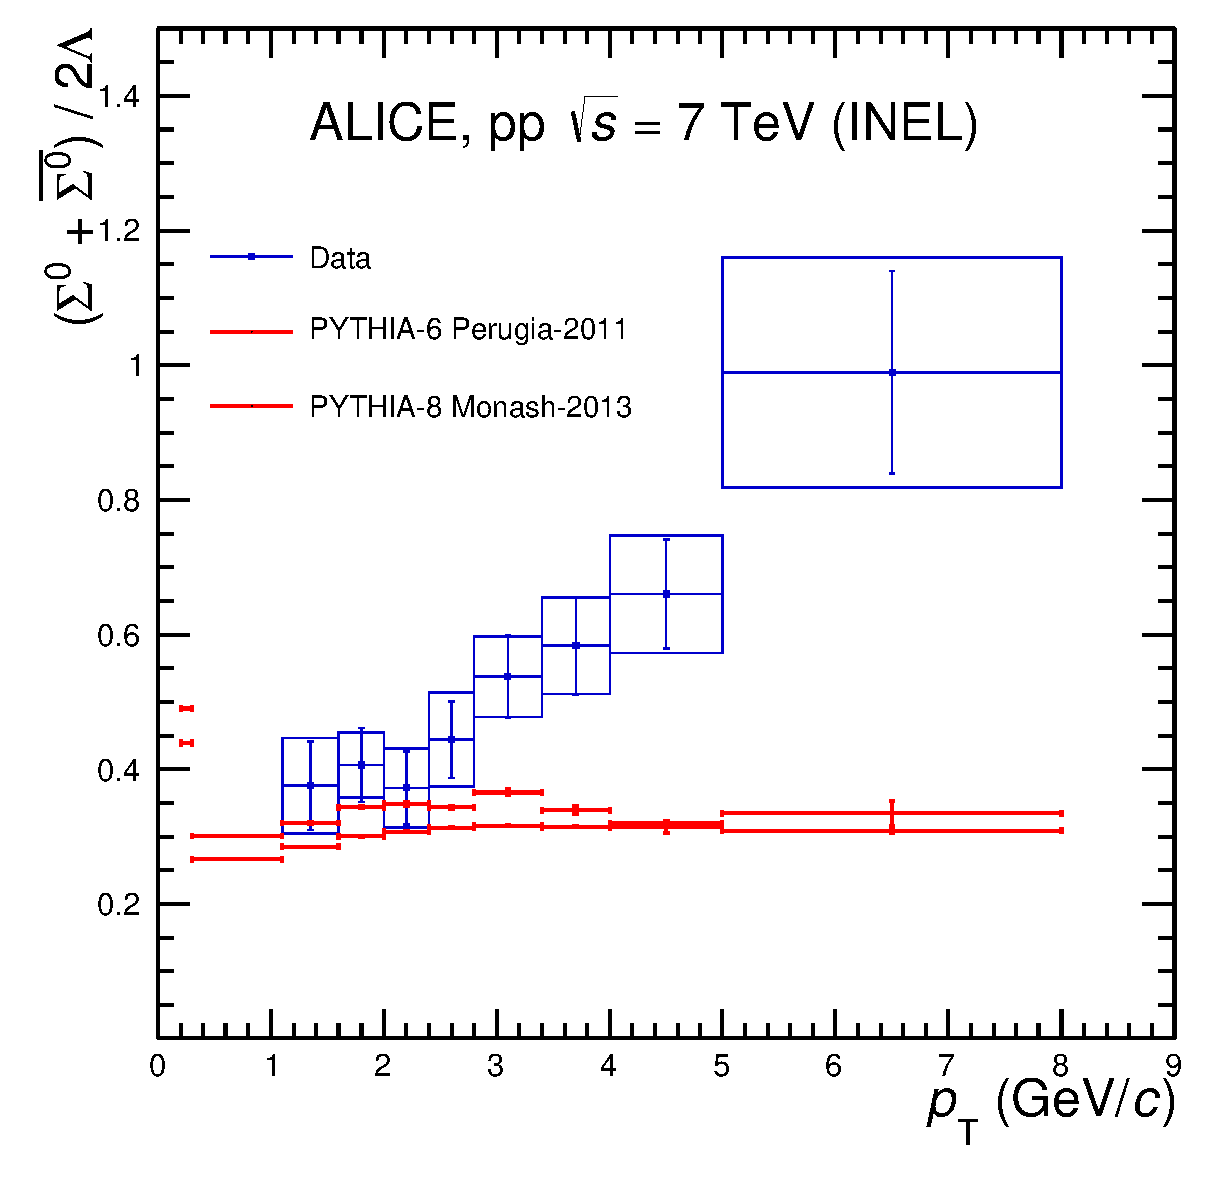
\includegraphics[width=10.cm]{Figure/ratio-Sigma0Lambda-7mar18.eps}

    \caption{ The differential ratios of \sig+\asig)/2 to \lam 
    from data~\cite{cite:ALICE-LF}  in the same bins of \pt (blue points). (The ratio (line) from the L\'{e}vy-Tsallis 
     curves based on \sig and \lam data is drawn     in full range of\pt. ???)
 The red points indicate the same ratios from PYTHIA 6-Perugia 2011 and magenta points from PYTHIA 8-Monash 2013, 
    respectively.
}
    \label{fig:siglam-ptdepratio}
\end{figure}

The integrated yield ratios of \sig to \lam from various collision systems at different enrgies are shown as a function
of $\sqrt{s}$ in Fig.~\ref{fig:SigLam-WorldData}. The integrated yield ratio measured with ALICE in pp collisions 
at $\sqrt{s} = 7$~TeV is $0.337  \pm 0.111(\mathrm{total}) = 0.337   \pm 0.051(\mathrm{stat}) 
\pm 0.099 (\mathrm{syst})$, where the extrapolation uncertainty is included into the systematic error. While yields 
of $\Sigma^0$ have been measured in many different collision systems at low and intermediate energies, there 
exist only few results in high energy collisions including the ALICE result. 
\blue{The relatively new and more precise COSY-TOF pp data  from Ref.
~\cite{cite:COSY-TOF,cite:Sigma0Phenomenology} see Fig.~\ref{fig:SigLam-WorldData}, have been 
published as the function of $\epsilon = \sqrt{s} -(m_p + m_K + m_{\Lambda,\Sigma^0})$ and correspond to
 $\sqrt{s} \approx 2 $ GeV/$c$. The cross section ratio $\frac{\Sigma^0}{\Lambda} \approx 0.45 \pm 0.05$.} \\
The STAR detector reconstructed the 
electromagnetic decay ($\Sigma^0 \to \Lambda + \gamma$) via the weak decay of the $\Lambda \to p + \pi^- $ and 
$\gamma$ conversions into $e^+ e^-$ pairs in the detector material \cite{cite:SigLamRatio-VanBuren,
 cite:Sigma0Phenomenology}. The cross section ratio $\Sigma^0/\Lambda = 0.16^{+0.41}_{-0.09}$ was thus obtained 
in minimum bias 0.2 TeV d+Au collisions. 
%\blue{ (See right plot in Fig.~\ref{fig:STAR-COSY} in Appendix~\ref{app:STAR}.)}
% or Fig.33 on p. 35 in the \sig analysis note in https://aliceinfo.cern.ch/Notes/node/562.
Note that STAR data with so large errors were published only in
a conference proceeding~\cite{cite:SigLamRatio-VanBuren} by the collaboration due to the limited statistics. 
\red{Note: The STAR result is, however, also cited in the regular paper~\cite{ cite:Sigma0Phenomenology}}
The most precise data are from L3 experiment~\cite{cite:L3, cite:L3_lambda}, where both $\Sigma^0$ and  $\Lambda$ have 
been measured as a product of Z boson decays, as shown in Fig.~\ref{fig:SigLam-WorldData}, where 
$\Sigma^0/\Lambda \approx 0.33 \pm 0.03$ (\red{This value is hardly confirmed from the two papers
~\cite{cite:L3, cite:L3_lambda} , and the phenomenology paper~\cite{ cite:Sigma0Phenomenology} DID NOT
cite this L3 value!}). These data in wide range of $\sqrt{s}$ support the convergence of the \sig/\lam-ratio as expected by \cite{cite:Sigma0Phenomenology}. 
High energy nuclear collisions are of particular interest for the final state interactions~\cite{cite:Sigma0Phenomenology} 
and the possibility of measuring isospin degeneracy factors from $\Sigma^0$ and $\Lambda$ yields and 
of opening new channels of hyperon production via partonic degrees of freedom \cite{cite:KochRafel-TimeEvolution}.

\begin{figure}[h!]
 \centering

 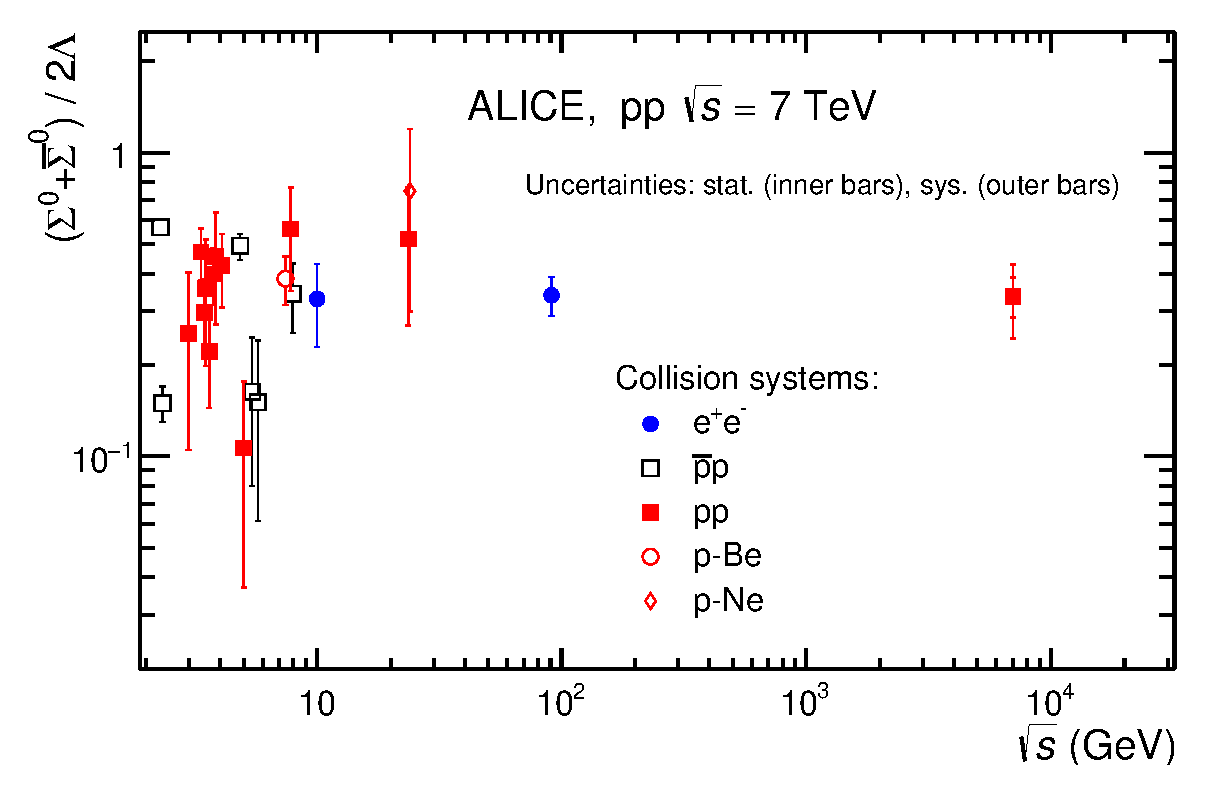
\includegraphics[width=15.0cm]{Figure/2017nov1-Sigma0-LambdaRatio-WorldData.eps}

  \caption{Energy dependence of \sig to \lam  cross section ratio
 \red{ Which points to include - to be discussed.}  }
  \label{fig:SigLam-WorldData}
\end{figure}

%%%%%%%%%%%%%% Chapter 4 : Conclusion %%%%%%%%%%%%
 \section{Conclusions}
 \label{sec:conclusion}

In summary, \sig (\asig) hyperons produced in pp collisions at $\sqrt{s} = 7 $ TeV are successfully reconstructed  
via electromagnetic decay to \lam (\alam) and $\gamma$. The \pt~distribution of (\sig + \asig)/2 is obtained
and compared with two different versions of PYTHIA generators, which both significantly underestimate the differential yields. 
So far no generator is found to explain the \sig yield produced in pp collisions at $\sqrt{s} = 7$~TeV.
Furthermore the differential yield ratios of \sig to \lam from data and the generators are compared and
the significant underestimates of \sig/\lam in both generators are observed in high \pt. 

The integrated yield ratio measured in pp collisions at $\sqrt{s} = 7$~TeV is (\sig+\asig)/2\lam=
$0.337  \pm 0.111(\mathrm{total}) = 0.337   \pm 0.051(\mathrm{stat})  \pm 0.099 (\mathrm{syst})$, 
where the systematic uncertainty includes the L\'{e}vy-Tsallis fits of \sig and \lam spectra extrapolated to the unmeasured low \pt.
So far this (\sig+\asig)/2\lam at the highest energy collision system uniquely contributes to consistency of an isospin degeneracy 
factor, 1/3 with the same ratios in various collisions at different energies from world-wide experiments. The current 
measurement represents a relevant baseline for further investigation in p-Pb and Pb-Pb collisions. 

 \newpage
\bibliography{mybib_v1}{}
\bibliographystyle{utphys}

\newpage
\appendix
\section{The ALICE Collaboration}
\label{app:collab}

\end{document}

